\starthis\section[能量-时间不确定度关系]{能量-时间不确定度关系} \label{sec:09.06} % 
% \makebox[5em][s]{} % 短题目拉间距

微观过程的某些性质常可用“能量-时间不确定度关系”来解释.这个“不确定度关系”的一般表达方式是
\eqshort
\begin{empheq}{equation}\label{eq96.1}
	\Delta E\Delta t\gtrsim\hbar
\end{empheq}\eqnormal
$\Delta E,\Delta t$分别代表能量和时间的不确定度.由于能量是力学量,$\Delta E$可以尽量按精确的意义理解,其严格定义是
\begin{empheq}{equation}\label{eq96.2}
	(\Delta E)^{2}=\overline{E^{2}}-\overline{E}^{2}
\end{empheq}\eqshort
而时间并非力学量,对于过程的时间不确定度,一般仅作量级估算.因此\eqref{eq96.1}式也仅在量级意义上使用.我们将先讨论几个典型实例,借以说明\eqref{eq96.1}式的正确性,然后再稍作理论探讨.


\exa 原子自发辐射,初态$\varPsi_{2}\rightarrow$终态$\varPsi_{1}(E_{2}-E_{1}>0)$设在$t=0$制备好大量处于初态$\varPsi_{2}$的原子,然后就测量辐射的光子能量$E=\hbar\omega$.设跃迁$\varPsi_{2}\rightarrow\varPsi_{1}$的平均寿命为$\tau$,有效测量大致在$t=\tau$前完成,可取$\Delta t\sim\tau$.被测量的光子,其空间分布范围大致是$\Delta x\lesssim c\tau$,因此有动量不定值$\Delta p\sim\frac{\hbar}{\Delta x}\gtrsim\frac{\hbar}{c\tau}$,和能量不定值$\Delta E=c\Delta p\gtrsim\frac{\hbar}{\tau}$.结论是:测到的光子能量$\hbar\omega$并不严格地等于原子跃迁前后的能级差$(E_{2}-E_{1})$,而有不确定度$\Delta E$,而$\Delta E$,$\Delta t$满足\eqref{eq96.1}式.

表面看来,以上结论与能量守恒定律有矛盾,其实不然.到测得光子时为止,原子在终态$\varPsi_{1}$中停留的时间是有限的$(t\lesssim\tau)$所以终态并非严格意义下的定态,其能量值并不严格等于$E_{1}$,而有分布宽$\Delta E\gtrsim\frac{\hbar}{\tau}$,初态也有类似的能级宽度.初、终态的能级宽度正是光子能量不确定度的来由.总之,如某状态只在有限时间内存在,它就不是严格的定态,而有能量分布$\Delta E$.

\exa 在粒子物理研究中发现,能够自行蜕变的不稳定粒子,其质量都有不确定度$\Delta m$,它与蜕变的平均寿命$\tau$有关系
\begin{empheq}{equation}\label{eq96.3}
	\Delta m\cdot\tau\sim\frac{\hbar}{c^{2}}
\end{empheq}\eqnormal
用能量-时间不确定关系\eqref{eq96.1}式容易解释这个关系,因为粒子质量与相对论性质的能量有关系$E=mc^{2}$,所以$\Delta E=c^{2}\Delta m$,而寿命$\tau$正是时间不确定度$(\Delta t\sim\tau)$.

\exa 在单频微扰作用下原子从初态$\varPsi_{k}$(能级$E_{k}$)向终态$\varPsi_{f}$(能级$E_{f}$)跃迁.跃迁概率由\eqref{eq92.5}式表示.考虑终态能量连续的情形,对于$F_{fk}$相同而能量互相不同的终态,跃迁概率与初终态能级差$(E_{f}-E_{k})=\hbar\omega_{fk}$有关系
\begin{empheq}{align*}
	|C_{f}(t)|^{2} &\propto\frac{[1-\cos(\omega_{fk}-\omega_{o})t]}{(\omega_{fk}-\omega_{o})^{2}}	\\
	&\propto \frac{\sin^{2}[(\omega_{fk}-\omega_{o})t/2]}{(\omega_{fk}-\omega_{o})^{2}}
\end{empheq}\eqshort
$|C_{f}(t)|^{2}-\omega_{fk}$关系如图\ref{fig.9-5}所示.$\omega_{fk}$的有效分布宽度大致可以确定为$\Delta\omega_{fk}\sim\frac{2\pi}{t}$,因此终态能量不确定度约为$\Delta E_{f}\sim\frac{2\pi\hbar}{t}$,即
\begin{empheq}{equation}\label{eq96.4}
	\Delta E_{f}\cdot\sim2\pi\hbar
\end{empheq}\eqnormal

\begin{figure}[!h]
	\centering
	\small
	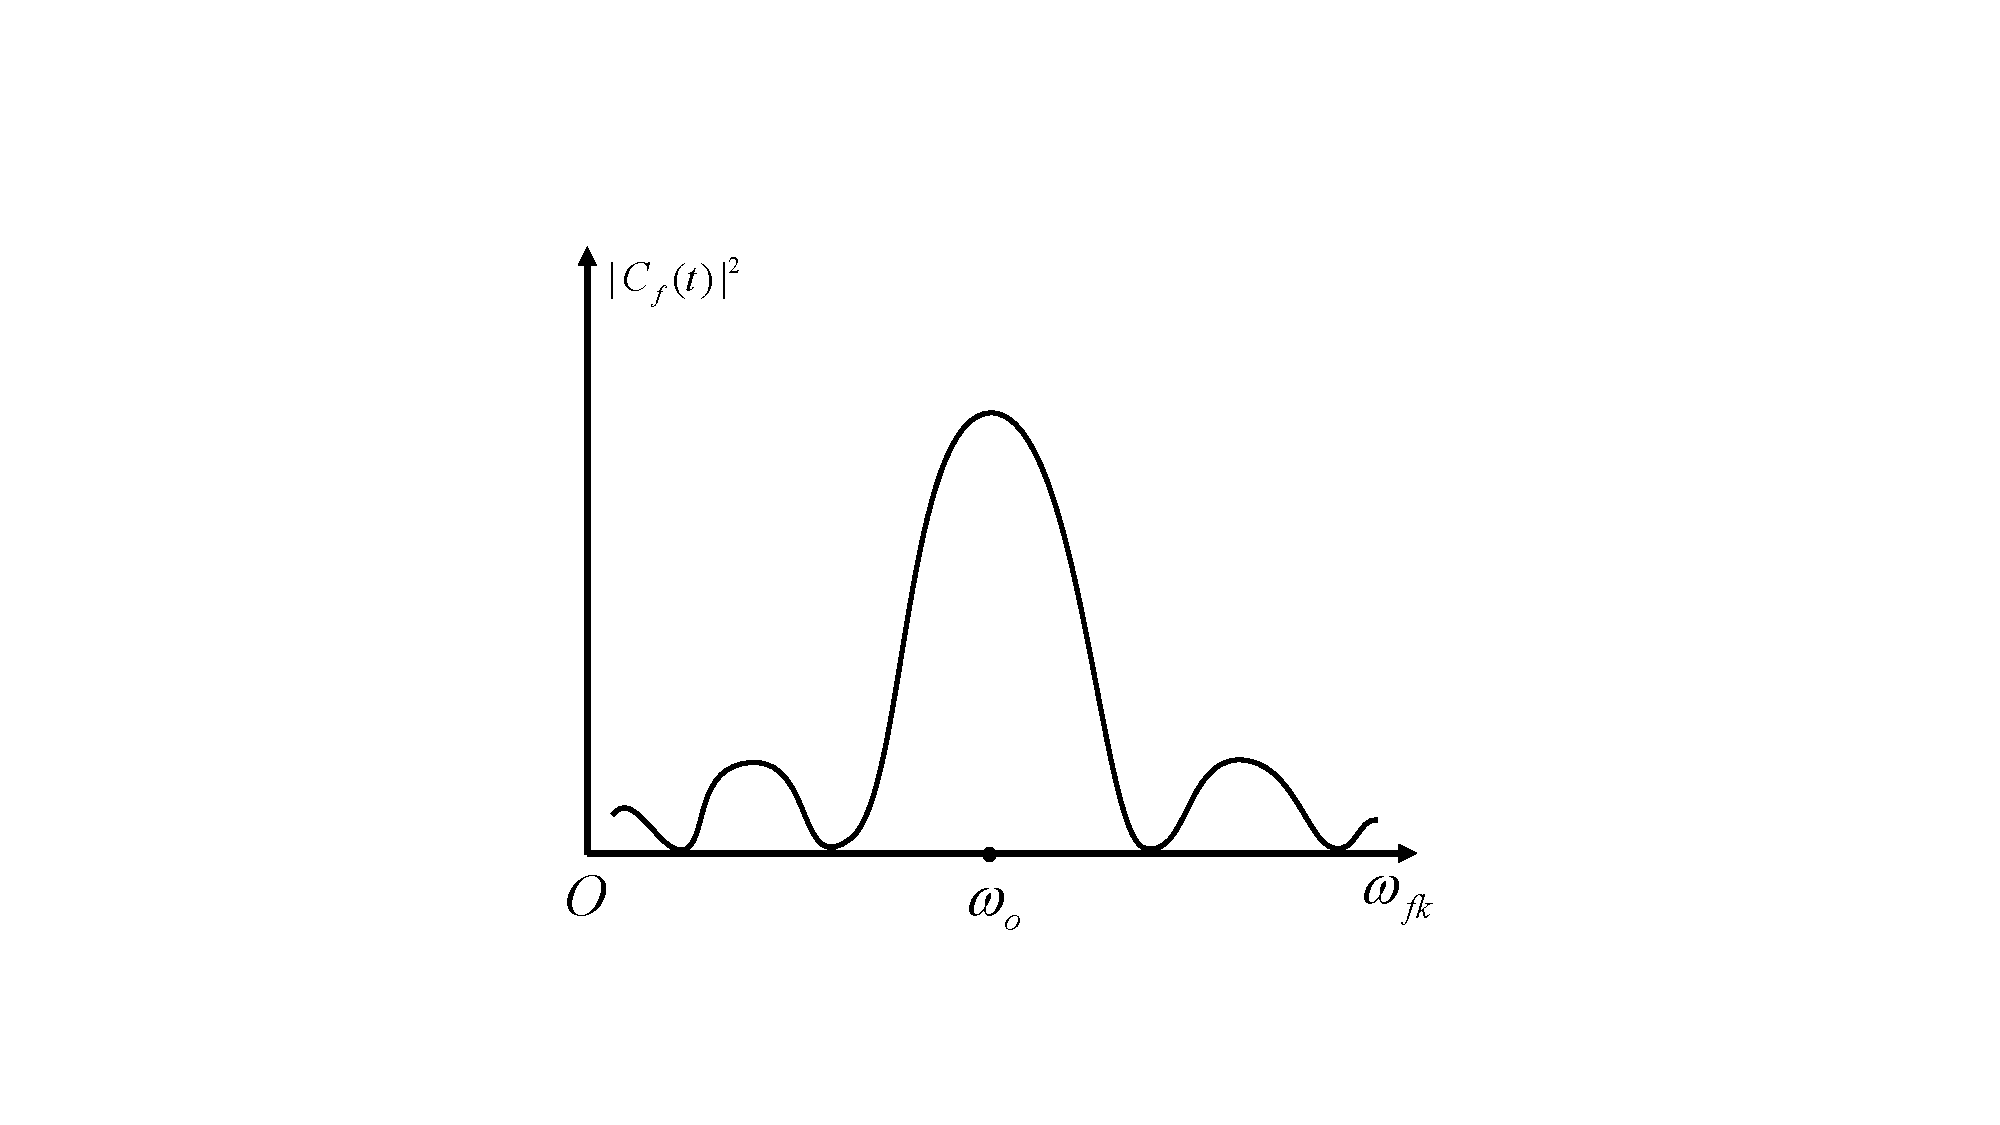
\includegraphics[width=5cm,clip]{QM file/figure/9-5}
	\caption{}\label{fig.9-5}
\end{figure}
\noindent 这里$t$相当于终态存在时间的不确定度,即$\Delta t$.造成终态能量不完全确定的原因是:微扰$H^{\prime}$既然只在有限时间内起作用,它实质上不是严格的单频微扰,其频谱宽度$\Delta\omega\gtrsim\frac{2\pi}{t}$,因此原子从$H^{\prime}$吸收的能量量子并不严格等于$\hbar\omega$,而有不确定度$\hbar\Delta\omega\gtrsim\frac{2\pi\hbar}{t}$,所以终态能量也有同样的不确定度.

在例1和例3中,$\Delta E$都很小,常可略去不计.例如例3,取$t\sim10^{-10}\si{s}$,则$\Delta E_{f}\sim\frac{\hbar}{t}\sim4\times10^{-5}\si{eV}$.$\S$\ref{sec:09.02}正是在忽略$\Delta E_{f}$的条件下,对跃迁速率作了近似处理,从而得出$E_{f}=E_{k}+\hbar\omega$的结论.但是例2中$\tau$有时非常小,$\Delta m$可以达到$m$的量级.

能量-时间不确定度关系的正确性是肯定的,对它的论证却并不统一.常见的一种论证是,取能量算符为$\hat{E}=i\hbar\frac{\partial}{\partial t}$,于是就有
\begin{empheq}{equation}\label{eq96.5}
	[t,\hat{E}]=[t,i\hbar\frac{\partial}{\partial t}]=-i\hbar
\end{empheq}\eqshort
再仿照$x-p_{x}$不确定关系的推导,得到
\begin{empheq}{equation*}
	\Delta E\cdot\Delta t\geqslant\frac{\hbar}{2}
\end{empheq}\eqnormal
这种论证显然不妥.我们姑且不去争论$t$是否可以作为算符对待,至少可以指出将$i\hbar\frac{\partial}{\partial t}$作为能量算符用于对易式的计算是不妥的,容易引申出种种谬论.例如,对于任何不显含$t$的算符$\hat{F}(\boldsymbol{r},\boldsymbol{p}$,显然有$\left[\hat{F},\frac{\partial}{\partial t}\right]=\frac{\partial\hat{F}}{\partial t}$,因此$F$是守恒量,等等.

利用狭义相对论中四维协变矢量的概念来论证能量-时间不确定关系也许是较好的办法.在相对论中,
\begin{empheq}{equation*}
	x_{\mu}=(x,y,z,ict),\quad p_{\mu}=\left(p_{x},p_{y},p_{z},\frac{iE}{c}\right)
\end{empheq}\eqshort
众所周知,利用$\hat{p_{x}}=-i\hbar\frac{\partial}{\partial x}$可以证明$x-p_{x}$不确定度关系:
\begin{empheq}{equation}\label{eq96.6}
	\Delta x\cdot\Delta p_{x}\geqslant\frac{\hbar}{2}
\end{empheq}
由于$\hat{p_{x}}=-i\hbar\frac{\partial}{\partial x}$也适用于相对论情形,所以\eqref{eq96.6}式也适用于相对论情形.$y-p_{y},z-p_{z}$间也有类似的不确定度关系.据此类推,$x_{4}=ict$与$p_{4}=\frac{iE}{c}$之间也应有不确定度关系:
\begin{empheq}{equation*}
	\Delta x_{4}\cdot\Delta p_{4}\geqslant\frac{\hbar}{2}
\end{empheq}
亦即
\begin{empheq}{equation} \label{eq96.7}
	\Delta t\cdot\Delta E\geqslant\frac{\hbar}{2}
\end{empheq}\eqnormal
在量级的意义上,\eqref{eq96.7}式与\eqref{eq96.1}式并无不同

